\documentclass{article}
\usepackage{fullpage}
\usepackage{graphicx}
\usepackage{hyperref}

\title{Aye-Aye Sleep Monitoring}
\author{Nathan Hui\\Engineers for Exploration\\UC San Diego\\nthui@ucsd.edu}
\begin{document}
\maketitle
\section{Introduction}
In 2020, the San Diego Zoo Wildlife Alliance\footnote{https://science.sandiegozoo.org/} and Engineers for Exploration\footnote{https://e4e.ucsd.edu} set on a path to develop a system for monitoring animals in the care of the San Diego Zoo, both at the Zoo in Balboa Park, the Safari Park in Escondido, and the Biodiversity Reserve behind the Safari Park.  The aim of this system was to provide 24/7 automated monitoring of animals with intelligent identification of abnormalities in behavior, which could indicate to animal care specialists the need to pay attention to certain things.  This system would also provide a corpus of data for future machine learning/artificial intelligence tools.

The first phase of this system was aimed at monitoring the aye-aye lemur (\textit{Daubentonia madagascariensis}) housed at the San Diego Zoo.  This species of lemur is nocturnal, which presents challenges to animal care specialists in understanding the effect being on exhibit during the day impacts the aye-aye's ability to sleep.  At a higher level, this also presents an opportunity to demonstrate a system capable of monitoring animals.
\section{System Requirements}
The key words ``MUST'', ``MUST NOT'', ``REQUIRED'', ``SHALL'', ``SHALL NOT'', ``SHOULD'', ``SHOULD NOT'', ``RECOMMEND'', ``MAY'', and ``OPTIONAL'' in this document are to be interpreted as described in \href{https://datatracker.ietf.org/doc/html/rfc2119}{RFC 2119}.

\begin{enumerate}
    \item The system MUST record video of the entire aye-aye enclosure.
    \item The system MUST record video of the entire inside of the aye-aye nesting box.
    \item The system SHOULD record audio from the inside of the aye-aye nesting box.
    \item The system MAY record additional data from the aye-aye nesting box that indicate sleep behavior for the aye-aye.
    \item The system MUST timestamp all data and store data in a central location.
    \item The system MUST provide a programmatic interface to access the data.
    \item The system MUST provide extensibility for additional sensor modalities, sensing, and automatic data processing.
    \item The system SHOULD automatically recover from faults with minimal loss of data.
    \item The system SHOULD provide for ensuring secure transfer of data.
\end{enumerate}
\section{System Architecture}
To solve this problem, we will use a central server as the end repository for all data, as well as for providing command and control.  We abstract all sensors as sensor nodes, which will represent the different sensor modalities.  For this phase of the design, we will connect the server and sensor nodes over Ethernet/WiFi. This is diagrammed in Figure \ref{fig:sys_diag}.

\begin{figure}[ht]
    \centering
    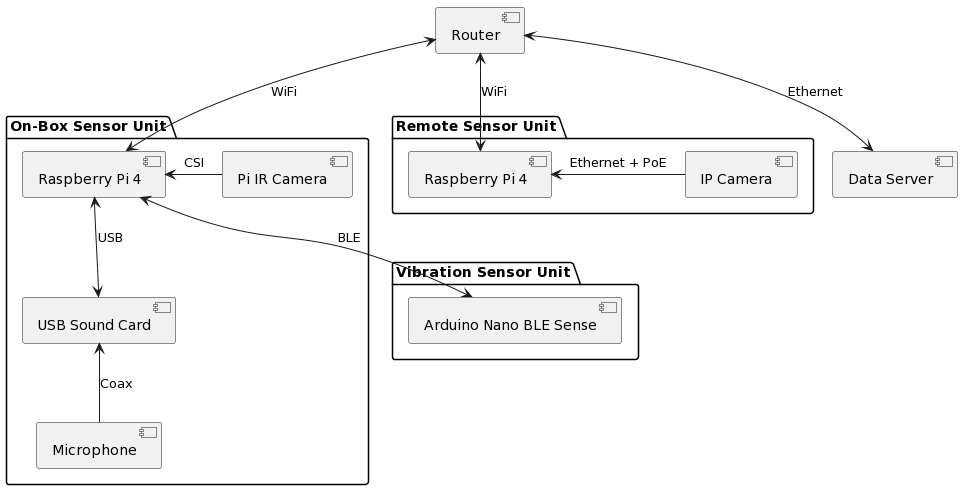
\includegraphics[width=0.8\textwidth]{images/System Diagram.png}
    \caption{System Diagram}
    \label{fig:sys_diag}
\end{figure}

For this to work, each major component is specified below.

\subsection{Data Server}
\begin{enumerate}
    \item The Data Server MUST aggregate all data from connected sensor nodes.
    \item The Data Server MUST provide an interface to access the aggregated data.
    \item The Data Server MUST add the following metadata to each data stream:
    \begin{enumerate}
        \item Originating sensor node
        \item Timestamp
    \end{enumerate}
    \item The Data Server MUST support nultiple sensor nodes that are dynamically added.
    \item The Data Server SHOULD support both encrypted and unencrypted sensor data.
    \item The Data Server SHOULD be capable of operating for 12 months without data offload or maintenance.
    \item The Data Server SHOULD be capable of automatically resuming operations after power loss.
    \item The Data Server MUST be able to monitor status of each Status Node.
\end{enumerate}

\subsection{On-Box Sensor Unit}
\begin{enumerate}
    \item The On-Box Sensor Unit MUST provide IR capable video data from the inside of the nesting box.
    \item The On-Box Sensor Unit MUST provide IR illumination when necessary.
    \item The On-Box Sensor Unit MUST provide audio data from the nesting box.
    \item The On-Box Sensor Unit SHOULD be capable of automatically resuming operations after power loss.
    \item The On-Box Sensor Unit MUST be powered from 60 Hz 120 VAC.
    \item The On-Box Sensor Unit MUST utilize WiFi connectivity.
\end{enumerate}

\subsection{Remote Sensor Unit}
\begin{enumerate}
    \item The Remote Sensor Unit MUST provide IR capable video data from its field of view over the enclosure.
    \item The Remote Sensor Unit SHOULD be capable of automatically resuming operations after power loss.
    \item The Remote Sensor Unit MUST be powered from 60 Hz 120 VAC.
    \item The Remote Sensor Unit MUST utilize WiFi connectivity.
\end{enumerate}

\subsection{Communications}
\begin{enumerate}
    \item Each Sensor Node MUST regularly indicate to the Data Server that it is alive.
    \item Each Sensor Node type MUST conform to a preset set of data types/formats.
    \item Sensor Nodes MUST regularly transmit data to the Data Server.
\end{enumerate}
\section{System and Component Design}
\subsection{Data Server}
The code for the Data Server is located at \url{https://github.com/UCSD-E4E/ASM-data-server}.  This is primarily based on an asyncio socket server, which creates individual handlers to manage each sensor node.  These handlers manage the communications between the server and node, and also handle spinning up and down relevant services in order to handle incoming data.

\subsection{Sensor Node}
The code for all sensor nodes is located at \url{https://github.com/UCSD-E4E/ASM-rpi-node}.  This is a common codebase for all sensor node types, since all of them do very similar things.  The base class provides communications abstractions, and handles all of the asynchronous receive/send.  Concrete subclasses handle the specific sensor bringup, configuration, and data management.
\end{document}